\documentclass[a4paper]{article}

\usepackage[italian]{babel}%traduzione parti generate automaticamente
\usepackage{geometry}
\geometry{a4paper,top=3cm,bottom=3cm,left=1.5cm,right=1.5cm} %dimensioni pagina benedetto
\usepackage[fontsize=13pt]{scrextend} % for change the fontsize, different from article class
\usepackage{fancyhdr}
\usepackage{indentfirst} %identatione nella prima frase del paragrafo
\usepackage{lastpage}
\usepackage{xcolor}
\usepackage{mdframed}
\usepackage[version=4]{mhchem}%per formule e equazioni chimiche
\usepackage{chemfig} %per formule 2D chimica
\usepackage{modiagram} % molecular orbital diagrams
\usepackage{wrapfig}
\usepackage{pgfplots}
\usepackage{floatrow}
\usepackage{tikz}
\usepackage{subcaption}
\usepackage{longtable} %Multi-page tables
\usepackage{graphicx}
\usepackage{amsthm}
\usepackage{amssymb}
\usepackage{tabularx}
\usepackage{array}
\usetikzlibrary{shapes.geometric, arrows, calc, patterns, positioning}%per flowchart
\usepackage{amsmath}
\usepackage{booktabs}
\usepackage{multicol}
\usepackage[font=scriptsize]{caption}%per didascalia immagini 
\usepackage{xstring} % per creare p e h phrase command
\usepackage{csquotes}
\usepackage[colorinlistoftodos,prependcaption,textsize=tiny]{todonotes}%solo per le note, utile per prendere appunti, se aggiungi "disable" si tolgono tutti dal pdf ma possono rimanere nel testo.
\usepackage{xargs} % Use more than one optional parameter in a new commands
\usepackage[autocite=superscript,style=chem-acs,articletitle,doi,url]{biblatex}%bibliografia, usare il comando \autocite perchè venga usato lo stile american chemical society
\usepackage{hyperref}%hyperlinks %package utilizzati per il documento
%File con config utili allo stile della relazione, in linea di massima qua non devi toccare nulla
%Nome e Cognome 
\def \nome {Nome}
\def \cognome {Cognome}

%page border and dimension
\geometry{a4paper,top=3cm,bottom=3cm,left=1.5cm,right=1.5cm}

%page style
\pagestyle{fancy}
\fancypagestyle{plain}{} %prima pagina uguale alle altre
\fancyhf{}
\rhead{\nome \ \cognome \\ Data consegna: xxxx}
\lhead{Relazione n° x \\ Classe: XE}
\rfoot{Pag. \thepage \hspace{1pt} di \pageref{LastPage}}
\lfoot{
\includegraphics[scale=0.1]{img/GitHub/qrcode_github.com.png} Template \LaTeX \;di M.Griot}
\setlength{\headheight}{22.54448pt}
\setlength{\footskip}{41.84514pt}

%noindent, se abilitata toglie l'identazione in tutto il documento
%\setlength{\parindent}{0pt}

%%%%%Colors
\definecolor{red}{RGB}{255,0,0}
\definecolor{orange}{RGB}{255,165,0}
\definecolor{blue}{RGB}{0,0,255}
\definecolor{green}{RGB}{143,206,0}

%%%%%%%%%% ToDo notes
% \usepackage[colorinlistoftodos,prependcaption,textsize=tiny,disable]{todonotes}
\newcommandx{\unsure}[2][1=]{\todo[linecolor=red,backgroundcolor=red!25,bordercolor=red,#1]{#2}}
\newcommandx{\change}[2][1=]{\todo[linecolor=orange,backgroundcolor=orange!25,bordercolor=orange,#1]{#2}}
\newcommandx{\info}[2][1=]{\todo[linecolor=blue,backgroundcolor=blue!25,bordercolor=blue,#1]{#2}}
\newcommandx{\improvement}[2][1=]{\todo[linecolor=green,backgroundcolor=green!25,bordercolor=green,#1]{#2}}
\newcommandx{\thiswillnotshow}[2][1=]{\todo[disable,#1]{#2}}

%per flowchart
\tikzstyle{startstop} = [rectangle, rounded corners, minimum width=3cm, minimum height=1cm,text centered, draw=black, fill=red!30]
\tikzstyle{io} = [trapezium, trapezium left angle=70, trapezium right angle=110, minimum width=3cm, minimum height=1cm, text centered, draw=black, fill=blue!30]
\tikzstyle{process} = [rectangle, minimum width=3cm, minimum height=1cm, text centered, draw=black, fill=orange!30]
\tikzstyle{decision} = [diamond, minimum width=3cm, minimum height=1cm, text centered, draw=black, fill=green!30]
\tikzstyle{arrow} = [thick,->,>=stealth]
\pgfplotsset{compat=1.18}

\usetikzlibrary{shapes.geometric, arrows, calc, patterns, positioning}%per flowchart

%per frasi H e P
\newcommand{\Hphrase}[1]{% 
    \IfEqCase{#1}{%
    %Pericoli Fisici
        {H200}{\textbf{H200} – Esplosivo instabile. [\textit{Cancellata}]}%
        {H201}{\textbf{H201} – Esplosivo; pericolo di esplosione di massa.}%
        {H202}{\textbf{H202} – Esplosivo; grave pericolo di proiezione.}%
        {H203}{\textbf{H203} – Esplosivo; pericolo di incendio, di spostamento d'aria o di proiezione.}%
        {H204}{\textbf{H204} – Pericolo di incendio o di proiezione.}%
        {H205}{\textbf{H205} – Pericolo di esplosione di massa in caso d'incendio.}%
        {H206}{\textbf{H206} – Pericolo d'incendio, di spostamento d'aria o di proiezione.}%
        {H207}{\textbf{H207} – Pericolo di incendio o di proiezione.}%
        {H208}{\textbf{H208} – Pericolo d'incendio.}%
        {H220}{\textbf{H220} – Gas altamente infiammabile.}%
        {H221}{\textbf{H221} – Gas infiammabile.}%
        {H222}{\textbf{H222} – Aerosol altamente infiammabile.}%
        {H223}{\textbf{H223} – Aerosol infiammabile.}%
        {H224}{\textbf{H224} – Liquido e vapori altamente infiammabili.}%
        {H225}{\textbf{H225} – Liquido e vapori facilmente infiammabili.}%
        {H226}{\textbf{H226} – Liquido e vapori infiammabili.}%
        {H227}{\textbf{H227} – Liquido combustibile.}%
        {H228}{\textbf{H228} – Solido infiammabile.}%
        {H229}{\textbf{H229} – Contenitore pressurizzato: può scoppiare se riscaldato.}%
        {H230}{\textbf{H230} – Può esplodere anche in assenza di aria.}%
        {H231}{\textbf{H231} – Può esplodere anche in assenza di aria a pressione e/o temperatura elevata.}%
        {H232}{\textbf{H232} – Spontaneamente infiammabile all'aria.}%
        {H240}{\textbf{H240} – Rischio di esplosione per riscaldamento.}%
        {H241}{\textbf{H241} – Rischio d'incendio o di esplosione per riscaldamento.}%
        {H242}{\textbf{H242} – Rischio d'incendio per riscaldamento.}%
        {H250}{\textbf{H250} – Spontaneamente infiammabile all'aria.}%
        {H251}{\textbf{H251} – Autoriscaldante; può infiammarsi.}%
        {H252}{\textbf{H252} – Autoriscaldante in grandi quantità; può infiammarsi.}%
        {H260}{\textbf{H260} – A contatto con l'acqua libera gas infiammabili che possono infiammarsi spontaneamente.}%
        {H261}{\textbf{H261} – A contatto con l'acqua libera gas infiammabili.}%
        {H270}{\textbf{H270} – Può provocare o aggravare un incendio; comburente.}%
        {H271}{\textbf{H271} – Può provocare un incendio o un'esplosione; molto comburente.}%
        {H272}{\textbf{H272} – Può aggravare un incendio; comburente.}%
        {H280}{\textbf{H280} – Contiene gas sotto pressione; può esplodere se riscaldato.}%
        {H281}{\textbf{H281} – Contiene gas refrigerato; può provocare ustioni o lesioni criogeniche.}%
        {H290}{\textbf{} – Può essere corrosivo per i metalli.}%
    %Pericoli per la Salute
        {H300}{\textbf{H300} – Letale se assimilato.}%
        {H301}{\textbf{H301} – Tossico se ingerito.}%
        {H302}{\textbf{H302} – Nocivo per ingestione.}%
        {H303}{\textbf{H303} – Può essere nocivo in caso di ingestione.}%
        {H304}{\textbf{H304} – Può essere letale in caso di ingestione e di penetrazione nelle vie respiratorie.}%
        {H305}{\textbf{H305} – \'E nocivo in caso di ingestione e di penetrazione nelle vie respiratorie.}%
        {H310}{\textbf{H310} – Letale per contatto con la pelle.}%
        {H311}{\textbf{H311} – Tossico per contatto con la pelle.}%
        {H312}{\textbf{H312} – Nocivo per contatto con la pelle.}%
        {H313}{\textbf{H313} – Può essere nocivo per contatto con la pelle.}%
        {H314}{\textbf{H314} – Provoca gravi ustioni cutanee e gravi lesioni oculari.}%
        {H315}{\textbf{H315} – Provoca irritazione cutanea.}%
        {H316}{\textbf{H316} – Provoca una lieve irritazione cutanea.}%
        {H317}{\textbf{H317} – Può provocare una reazione allergica cutanea.}%
        {H318}{\textbf{H318} – Provoca gravi lesioni oculari.}%
        {H319}{\textbf{H319} – Provoca grave irritazione oculare.}%
        {H320}{\textbf{H320} – Provoca irritazione oculare.}%
        {}{\textbf{} – }%
        {}{\textbf{} – }%
        {}{\textbf{} – }%
        {H341}{\textbf{H341} – Sospettato di provocare alterazioni genetiche.}%
        {H350}{\textbf{H350} – Può provocare il cancro.}%
        {H351}{\textbf{H351} – Sospettato di provocare il cancro.}%
        {H361}{\textbf{H361} – Sospettato di nuocere alla fertilità o al feto.}%
        {H372}{\textbf{H372} – Provoca danni agli organi in caso di esposizione prolungata o ripetuta.}%
        {}{\textbf{} – }%
        {}{\textbf{} – }%
        {}{\textbf{} – }%
        {}{\textbf{} – }%
        {}{\textbf{} – }%
        {}{\textbf{} – }%
        {}{\textbf{} – }%
        {}{\textbf{} – }%
        {}{\textbf{} – }%
        {}{\textbf{} – }%
        {}{\textbf{} – }%
        {}{\textbf{} – }%
        {}{\textbf{} – }%
        {}{\textbf{} – }%
        {}{\textbf{} – }%
        {}{\textbf{} – }%
        {}{\textbf{} – }%
        {}{\textbf{} – }%
        {}{\textbf{} – }%
        {}{\textbf{} – }%
        {}{\textbf{} – }%        
        % you can add more cases here as desired
    }[\PackageError{Hphrase}{Undefined option to Hphrase: #1}]%
}%-

\newcommand{\Pphrase}[1]{% 
    \IfEqCase{#1}{%
    %Consigli di prudenza di carattere generale
        {P101}{\textbf{P101} – In caso di consultazione di un medico, tenere a disposizione il contenitore o l'etichetta del prodotto.}%
        {P102}{\textbf{P102} – Tenere fuori dalla portata dei bambini.}%
        {P103}{\textbf{P103} – Leggere l'etichetta prima dell'uso.}%
        {}{\textbf{} – }%
        {P201}{\textbf{P201} – Procurarsi le istruzioni prima dell'uso.}%
        {P202}{\textbf{P202} – Non manipolare prima di avere letto e compreso tutte le avvertenze.}%
        {P260}{\textbf{P260} – Non respirare la polvere/i fumi/i gas/la nebbia/i vapori/gli aerosol.}%
        {P261}{\textbf{P261} – Evitare di respirare la polvere/i fumi/i gas/la nebbia/i vapori/gli aerosol. [modificato]}%
        {P264}{\textbf{P264} – Lavare accuratamente … dopo l’uso.}%
        {P270}{\textbf{P270} – Non mangiare, né bere, né fumare durante l'uso.}%
        {P280}{\textbf{P280} – Indossare guanti/indumenti protettivi/proteggere gli oc­chi/proteggere il viso/pro­teggere l'udito/... [modificato]}%
        {P281}{\textbf{P281} – [soppresso]}%
        {P305 + P351 + P338}{\textbf{P305 + P351 + P338} –  IN CASO DI CONTATTO CON GLI OCCHI: sciacquare accuratamente per parecchi minuti. Togliere le eventuali lenti a contatto se è agevole farlo. Continuare a sciacquare.}%
        {P302 + P352}{\textbf{P302 + P352} – IN CASO DI CONTATTO CON LA PELLE: Lavare abbondantemente con acqua/… [modificato]}%
        {}{\textbf{} – }%
        {}{\textbf{} – }%
        {}{\textbf{} – }%
        {}{\textbf{} – }%
        {}{\textbf{} – }%
        {}{\textbf{} – }%
        {}{\textbf{} – }%
        {}{\textbf{} – }%
        {}{\textbf{} – }%
        {}{\textbf{} – }%
        {}{\textbf{} – }%
        {}{\textbf{} – }%
        {}{\textbf{} – }%
        {}{\textbf{} – }%
        {}{\textbf{} – }%
        {}{\textbf{} – }%
        {}{\textbf{} – }%
        {}{\textbf{} – }%
        {}{\textbf{} – }%
        {}{\textbf{} – }%
        {}{\textbf{} – }%
        {}{\textbf{} – }%
        {}{\textbf{} – }%
        {}{\textbf{} – }%
        {}{\textbf{} – }%
        {}{\textbf{} – }%
        {}{\textbf{} – }%
        {}{\textbf{} – }%
        {}{\textbf{} – }%
        {}{\textbf{} – }%
        {}{\textbf{} – }%
        {}{\textbf{} – }%
        {}{\textbf{} – }%
        {}{\textbf{} – }%
        % you can add more cases here as desired
    }[\PackageError{Pphrase}{Undefined option to Pphrase: #1}]%
}%-
% https://it.wikipedia.org/wiki/Indicazioni_di_pericolo_H
% https://pubchem.ncbi.nlm.nih.gov/ghs/
% https://unece.org/transport/standards/transport/dangerous-goods/ghs-rev9-2021
% https://unece.org/sites/default/files/2021-09/GHS_Rev9E_0.pdf-

%set title and author in pdf information
\hypersetup{pdftitle={Template Example}, pdfauthor={\cognome \; \nome}}

%aggiunge il file di bibliografia per fare le citazioni
\addbibresource{bibliography.bib} %Import the bibliography file



 %file con settaggi

\begin{document}
\maketitle %crea il titolo

\noindent\rule{1\textwidth}{0.5pt}
    \begin{abstract}
        La relazione tecnica che conclude un'esperienza ha lo scopo di comunicare gli obbiettivi del proprio lavoro, le modalità con cui si è svolto e i risultati ottenuti. 
        
        Essa dev'essere redatta in modo tale che chiunque possa riprodurre l'esperimento realizzato e confrontare i risultati.
        
        Per questo motive la relazione tecnica deve essere articolata, nell'ordine, nei seguenti punti. Ogni sezione viene analizzata e spiegata cercando di dare dei suggerimenti per la stesura.
    \end{abstract} 
\noindent\rule{1\textwidth}{0.5pt} %da eleiminare
\section{Objective}
Sometimes it is referred to as Purpose.

It is useful to express the objectives of the experiment (however, sometimes it is not necessary because it is already indicated in the title).
\info[inline]{example "Purification and recrystallization of benzoic acid after contaminating it with activated carbon."}

\section{Principio del metodo}
A volte è indicato come Sommario o Principio del metodo.

Fa riferimento a tutti i principi teorici su cui si basa l'esperienza e a come essi si sono utilizzati per raggiungere gli obbiettivi prefissati.Qui devi mettere tutti i concetti teorici necessari a comprendere la relazione, devi spiegare tutto quello che merita essere spiegato. Solitamente se hai già scritto delle relazioni puoi pensare di omettere alcune parti che potrebbero ripetersi e snellire un po' il tutto.
\section{Instruments}
Sometimes it is referred to as Equipment.

Specifies the type of glassware and instrumentation required by the experiment and reports all the technical data deemed significant.
\info[inline]{e.g. the tolerance and capacity of the glassware.}

All the instruments used during the experiment must be listed in detail. Also the type of glassware (pyrex or not, the class of the glassware, capacity and sensitivity are important).
In practice, the technical data of the instruments used must be entered.

You can use a bulleted list and, if necessary, nest one inside to better group the instruments.

e.g.
\begin{itemize}
    \item Instruments:
    \begin{itemize}
        \item Microscope slide;
        \item Bunsen burner;
        \item Inoculating loop;
        \item Wooden tongs;
        \item Burette, capacity 25 mL and tolerance 0.05 mL;
        \item ...
    \end{itemize}
    \item Media:
    \begin{itemize}
    \item Malt Agar;
    \item Nutrient Agar.
    \end{itemize}
    \item Dyes
    \begin{itemize}
        \item Methylene blue;
        \item Gentian violet.
    \end{itemize}
\end{itemize}

When the list is particularly long it would be better to create two columns, it makes the report less papyrus-like and fills the spaces better.

e.g.
\begin{multicols}{2}
\begin{itemize}
    \item Instruments:
    \begin{itemize}
        \item Microscope slide;
        \item Bunsen burner;
        \item Inoculating loop;
        \item Wooden tongs;
        \item ...
    \end{itemize}
    \item Media:
    \begin{itemize}
    \item Malt Agar;
    \item Nutrient Agar.
    \end{itemize}
    \item Dyes
    \begin{itemize}
        \item Methylene blue;
        \item Gentian violet.
    \end{itemize}
\end{itemize}
\end{multicols}

Another alternative is to create a table and put the various instruments used inside, divided by columns.

e.g.
\begin{center}
   \begin{tabular}{l|c|r}
   \toprule
     \textbf{Instruments} &  \textbf{Media} & \textbf{Dyes}\\
    \midrule
     Microscope slide & Malt Agar & Methylene blue\\
     Bunsen burner & Nutrient Agar & Gentian violet\\
     Inoculating loop & & \\
     Wooden tongs & & \\
     ... & & \\
     \bottomrule
    \end{tabular} 
\end{center}

\section{Reagenti}
Indica il tipo e le caratteristiche dei reagenti  impiegati (è essenziale segnalare la concentrazione delle soluzioni e, per i solidi, il grado di purezza).
Nel caso i reagenti disponessero di una scheda di sicurezza è buona norma riportare in maniera sintetica tali informazioni come pittogrammi, frasi H e P, i DPI necessari la TLV.

A questo scopo viene mostrato anche come mettere le equazioni e formule chimiche con un pacchetto apposito:
\begin{itemize}
    \item \ce{H3PO4} 0.3 M 25 mL
\end{itemize}

\begin{table}[!ht]
    \scriptsize
    \centering
    \begin{tabularx}{\textwidth}{m{0.15\textwidth}|m{0.2\textwidth}|m{0.23\textwidth}|m{0.17\textwidth}|m{0.13\textwidth}}
        \toprule
        \textbf{Composto}                                                                                                                                                                                                                 & \textbf{Formula di struttura}                                                 & \textbf{Frasi H e P}       & \textbf{Pittogrammi} & \textbf{DPI} \\
        \midrule
        \ce{H2O2}                                                                                                                                                                                                                         & \begin{center}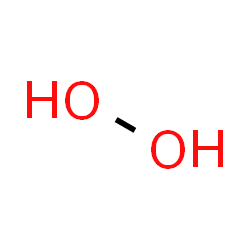
\includegraphics[width=3cm,scale=0.4]{img/763.png} \end{center} &
        H: H271, H302, H314 e H332.

        P: P210, P220, P221, P260, P261, P264, P270, P271, P280, P283, P301+P312, P301+P330+P331, P303+P361+P353, P304+P312, P304+P340, P305+P351+P338, P306+P360, P310, P312, P321, P330, P363, P370+P378, P371+P380+P375, P405, e P501. & \begin{center} \begin{tabular}{cc}
                
\includegraphics[scale=0.15]{img/pittogrammi/Flammable.png} & 
\includegraphics[scale=0.15]{img/pittogrammi/Explosive.png} \\
                
\includegraphics[scale=0.15]{img/pittogrammi/Flammable.png} & 
\includegraphics[scale=0.15]{img/pittogrammi/Explosive.png}
            \end{tabular}\end{center}                          & guanti, occhiali e visiera                                       \\
        \bottomrule
    \end{tabularx}
    \caption{Tabella con i composti chimici utilizzati nell'esperienza, le frasi P e H vengono riportate per esteso al fondo della relazione.} % da modificare
    \label{tab:tab1} % da modificare
    \normalsize
\end{table}

\newpage
Tabella precedente con i TLV (threshold limit value) che sono valori di concentrazione di sostanze aerodisperse, più o meno tossiche, al di sotto delle quali la maggior parte dei lavoratori può rimanere esposta ripetutamente tutti giorni senza effetti dannosi per la salute.

\begin{table}[!ht]
    \centering
    \scriptsize
    \begin{tabularx}{1\textwidth}{m{0.15\textwidth}|m{0.15\textwidth}|m{0.2\textwidth}|m{0.12\textwidth}|m{0.1\textwidth}|m{0.13\textwidth}}
        \toprule
        \textbf{Composto}                                                                                                             & \textbf{Formula di struttura}                                                            & \textbf{Frasi H e P}                         & \textbf{Pittogrammi} & \textbf{DPI} & \textbf{TLV [ppm]} \\
        \midrule
        \ce{H2O2}                                                                                                                     & \begin{center}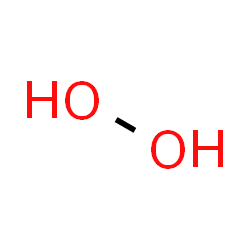
\includegraphics[width=0.15\textwidth,scale=0.4]{img/763.png} \end{center} & \Hphrase{H271} \Hphrase{H302} \Pphrase{P261} &
        \begin{tabular}{c}
            
\includegraphics[scale=0.15]{img/pittogrammi/Flammable.png} \\ 
\includegraphics[scale=0.15]{img/pittogrammi/Explosive.png} \\
            
\includegraphics[scale=0.15]{img/pittogrammi/Flammable.png} \\ 
\includegraphics[scale=0.15]{img/pittogrammi/Explosive.png}
        \end{tabular} & guanti, occhiali e visiera                                                               & LTEL: 100

        STEL: 200                                                                                                                                                                                                                                                                                                                          \\
        \bottomrule
    \end{tabularx}
    \caption{Tabella con i composti chimici utilizzati nell'esperienza, le frasi P e H vengono riportate per esteso al fondo della relazione. Ricorda che: Long-term Exposure Limit (LTEL) Values e Short-term Exposure Limit (STEL) Values} % da modificare
    \label{tab:tab2} % da modificare
    \normalsize
\end{table}

Oppure, in alcuni casi, è necessaria una tabella differente come la seguente.

Esprime i rapporti stechiometrici, le masse e le rese, utili nelle reazioni di sintesi quando si deve capire il meccanismo e quest'ultimo può variare in base alle concentrazioni dei reagenti.

\begin{table}[ht]
    \centering
    \scriptsize
    \begin{tabularx}{1\textwidth}{X|X|X|X|X|X|X|X|X}
        \toprule
        Sostanza & Massa molecolare\newline[g/mol] & Moli\newline[mol] & Rapporto stechiometrico & Massa\newline[g] & Volume\newline[mL] & Resa\newline[\%] & Frasi H & Frasi P \\
        \midrule
        A        & B                               & C                 & D                       & E                & F                  & G                & H       & I       \\
        \bottomrule
    \end{tabularx}
    \caption{Tabella per sintesi}
    \label{tab:tab3}
    \normalsize
\end{table}

\begin{table}[ht]
    \centering
    \scriptsize
    \begin{tabularx}{1\textwidth}{X|X|X|X|X|X|X}
        \toprule
        Composto & Struttura & Aspetto          & Rischi  & Protezioni & TLV/TWA     & Smaltimento                         \\
        \midrule
        \ce{H2O} &           & liquido incolore & nessuno & nessuna    & irrilevante & semplicemente gettare nel lavandino \\
        \midrule
        \ce{H2O} &           & liquido incolore & nessuno & nessuna    & irrilevante & semplicemente gettare nel lavandino \\
        \midrule
        \ce{H2O} &           & liquido incolore & nessuno & nessuna    & irrilevante & semplicemente gettare nel lavandino \\
        \midrule
        \ce{H2O} &           & liquido incolore & nessuno & nessuna    & irrilevante & semplicemente gettare nel lavandino \\
        \bottomrule
    \end{tabularx}
    \caption{Altro modello di tabella.}
    \label{tab:my_label}
\end{table}

Per i DPI si è costretti a cercare il nome del composto e scrivere di seguito scheda di sicurezza su un qualsiasi motore di ricerca e cercando il risultato più recente.

\info[inline]{es. acido benzoico scheda di sicurezza.}

Ricordarsi il produttore, facendo una foto in laboratorio del contenitore, può accelerare il lavoro ed essere più corretti in quanto le informazioni potrebbero non sempre essere uguali.
In fondo alla scheda si trova, oltre alle informazioni sui DPI, altre varie informazioni utili.

\section{Procedimento}
Riferisce la procedura  operativa seguita. Spesso si completa con un disegno schematico dell'attrezzatura utilizzata, quando è utile per descrivere le istruzioni di assemblaggio della stessa.
Qui bisogna spiegare in maniera sintetica ma esaustiva tutti i passaggi svolti durante l'esperimento.

Sono ammessi anche dei commenti o delle osservazioni, se hanno un senso. Nel caso di particolari non menzionati nella procedura ma osservati durante l'esperienza come l'aumento di temperatura in una reazione che impedirebbe di tenere in mano una provetta da saggio.

\info[inline]{es. Aggiungere la lega di di Devarda. \textit{Attenzione! Dopo l'aggiunta il contenuto della provetta raggiunge alte temperature, meglio svolgere l'operazione vicino ad un bancone e con una scarabattola per posare la provetta.}}


Un altra cosa che puoi aggiungere è un flowchart che riassuma i passaggi, questo può servire anche per aver chiaro il procedimento e eventualmente studiare.


\section{Reazioni}
Anche detto meccanismo di reazione.

Se le esperienze prevedono delle reazioni queste vanno riportate e spiegate, è una delle parti fondamentali in un esperimento chimico.

\ce{2H2O^2+}

\ce{H2O <=> 2H+ + 2O-}

\ce{CH#CH}

\ce{CH2=CH2}

\ce{CH3-CH3}

\ce{A ->[C] B}
\section{Dati e Calcoli}
In questa sezione si deve raccogliere tutti i risultati che si sono ottenuti. Vanno bene foto, tabelle di dati e osservazioni personali. I dati sarebbe buono che vengano raccolti in tabella se sono in numero sufficiente. 
\'E anche vero che si possono unire le due sezioni dei dati per rendere più discorsivo il tutto.

In questa sezione si devono anche scrivere tutte le formule che si usano per i calcoli indicando cosa servono e le loro unità di misura.

Ci sono due modi per impostare le cose, nel primo modo si scrivono prima tutte le formule e poi dopo si svolgono i conti con i propri dati, oppure in alternativa, si scrive la formula e poi subito dopo il conto relativo. Se si sceglie di fare il secondo metodo si potrebbe usare una tabella

\textbf{Primo metododo:}
Le moli si trovano tramite la seguente formula:
\begin{equation}
   n=M[mol/L]\cdot V[L]=n [mol] 
   \label{eq:mol} %questo ti serve per citare le equazioni, in questa sezione non è molto utile ma nei cenni teorici ti può aiutare a scrivere meglio le frasi senza intortarti da solo
\end{equation}
E ora si svolge il calcolo sui propri dati, in questo caso aggiungo un "*" all'ambiente per togliere i numeri:
\begin{equation*}
   n=\frac{0.5\cdot 25}{1000}=0.0125 [mol] 
\end{equation*}
Si divide per  1000 percheè il volume è stato espresso in mL.

\textbf{Nel secondo modo invece:}
\begin{center}
    \begin{tabularx}{0.9\textwidth}{XcX}
    Formule & & Calcoli\\
    \midrule
    $n=M[mol/L]\cdot V[L]=n [mol] $ &$\rightarrow$& $ n=\frac{0.5\cdot 25}{1000}=0.0125 [mol] $\\
    $n=M[mol/L]\cdot V[L]=n [mol] $ &$\rightarrow$& $ n=\frac{0.5\cdot 25}{1000}=0.0125 [mol] $\\
    $n=M[mol/L]\cdot V[L]=n [mol] $ &$\rightarrow$& $ n=\frac{0.5\cdot 25}{1000}=0.0125 [mol] $\\
    $n=M[mol/L]\cdot V[L]=n [mol] $ &$\rightarrow$& $ n=\frac{0.5\cdot 25}{1000}=0.0125 [mol] $\\
    $n=M[mol/L]\cdot V[L]=n [mol] $ &$\rightarrow$& $ n=\frac{0.5\cdot 25}{1000}=0.0125 [mol] $\\
    \end{tabularx}
\end{center}
Bisogna trovare il modo per distanziare un po' il testo in verticale ma ci può stare.

\subsection{Dati sperimentali}
Vanno riportati \textit{tutti} i dati sperimentali, evidenziando se necessario, quelli "aberranti", cioè da scartare sulla base si un analisi statistica.
Laddove possibile, è bene raccogliere i dati sotto forma di tabelle.
\vspace{1ex}
\begin {center}
\begin{tabular}{c|c}
     Esperimento &  Risultato\\
     1 & 10\\
     2 & 15\\
     3 & ...
\end{tabular}
\end {center}

\subsection{Elaborazione dei dati}
(Se necessario anche grafica): riporta i calcoli effettuati a partire dai risultati sperimentali, indicando le relazioni matematiche utilizzate. L'elaborazione può consistere anche nella costruzione di diagrammi o grafici.
A volte essa prevede anche il trattamento statistico dei dati.

Plotting from data:
\begin{center}
\vspace{2ex}
\begin{figure}[!ht]
    \centering
    \begin{tikzpicture}
        \begin{axis}[
            title={Temperature dependence of CuSO\(_4\cdot\)5H\(_2\)O solubility},
            xlabel={Temperature [\textcelsius]},
            ylabel={Solubility [g per 100 g water]},
            xmin=0, xmax=100,
            ymin=0, ymax=120,
            xtick={0,20,40,60,80,100},
            ytick={0,20,40,60,80,100,120},
            legend pos=north west,
            ymajorgrids=true,
            grid style=dashed,
            ]

            \addplot[
                color=blue,
                mark=square,
                ]
                coordinates {
                (0,23.1)(10,27.5)(20,32)(30,37.8)(40,44.6)(60,61.8)(80,83.8)(100,114)
                };
                \legend{CuSO\(_4\cdot\)5H\(_2\)O}
                
            \end{axis}
        \end{tikzpicture}
    \caption{Grafico di solubilità del solfato di rame in base alla temperatura.}
    \label{plt:1}
\end{figure}

\end{center}
\newpage


\section{Conclusioni}
Qui trovano spazio eventuali note dell'operatore riguardanti aspetti procedurali e la sua valutazione dei risultati precedentemente elaborati, in riferimento agli obiettivi previsti dall'esperienza. \'E importante segnalare eventuali anomalie riscontrate nei confronti della metodica utilizzata, nonchè i passaggi che hanno causato difficoltà (in particolare sotto il profilo di sicurezza).

Ultima sezione della relazione, forse è la più importante insieme ad obbiettivo e procedimento. In questa parte devi trare le conclusioni dell'esperimento. 
\begin{itemize}
    \item Esito (riuscito-fallito);
    \item Risultato (sensato-assurdo), confrontando l'esito con quelli riportati in letteratura o tramite conti ricavati dalla letteratura;
    \item Osservazioni tue personali sui passaggi che potresti aver sbagliato o che magari ritieni di aver fato nella maniera migliore rispetto alle indicazioni del prof, spiegare e motivare.
\end{itemize}
\section{Bibliografia}
Alle superiori non serve ma in futuro, se continui, sarà essenziale citare le fonti che hai usato per stendere un qualsiasi tipo di elaborato scritto ( ad eccezione del materiale del docente). Questa sezione serve proprio a quello, ti permette di raccogliere i siti e gli articoli da cui hai preso le informazioni (soprattutto quelle dei cenni teorici). 

Ti può servire, nel caso tu volessi recuperare le fonti da cui hai preso le cose per studiare o nel caso qualcuno ti dicesse che hai sbagliato a scrivere qualcosa.

Esempio di citazione.\autocite{einstein}

\printbibliography %Prints bibliography
\section*{\quad \   Frasi H e P}%remove "\quad \   " if you use bibliography

Questa sezione è un'alternativa, nel caso non si vogliano riportare tutte le frasi P e H nelle tabelle dei reagenti si possono fare qui.
Vengono riportati i seguenti link, \href{https://it.wikipedia.org/wiki/Indicazioni_di_pericolo_H}{\textcolor{blue}{H}} e \href{https://it.wikipedia.org/wiki/Consigli_P}{\textcolor{blue}{P}}, che riguardano le frasi P e H in modo da avere un elenco ordinato.

Questo template incorpora anche un piccolo file che si occupa di riportare le frasi tramite un comando, basta inserire il numero e in automatico verrà riportato il testo in modo da rendere il file \LaTeX\ più snello.

\begingroup
\begin{multicols}{2}
\scriptsize
\subsection*{Pericoli fisici}
\begin{itemize}
    \item \Hphrase{H200}
    \item \Hphrase{H240}
\end{itemize}
\subsection*{Pericoli per la salute}
\begin{itemize}
    \item \Hphrase{H315}
    \item \Hphrase{H318}
    \item \dots
\end{itemize}
\subsection*{Consigli di prudenza di carattere generale}
\begin{itemize}
    \item \Pphrase{P101}
    \item \dots
\end{itemize}
\end{multicols}
\endgroup




\newpage
\section*{link utili}

Piccola raccolta di link e pagine utili per scrivere la relazione.
\begin{footnotesize}
\begin{multicols}{2}
\begin{itemize}
    \item \href{https://molview.org/}{\textcolor{blue}{MolView}}: sito ottimo per avere immagini 2D e 3D dei composti chimici;
    \item \href{https://echa.europa.eu/it/regulations/clp/clp-pictograms}{\textcolor{blue}{ECHA-clp-pictograms}}: sito europeo per l'etichettatura e registrazione delle sostanze chimiche;
    \item \href{https://echa.europa.eu/it/information-on-chemicals/cl-inventory-database}{\textcolor{blue}{ECHA-cl-inventory-databas}}: per quanto riguarda le informazioni dei composti e la loro classificazione in europa;
    \item \href{https://pubchem.ncbi.nlm.nih.gov/}{\textcolor{blue}{PubChem}}: PubChem is the world's largest collection of freely accessible chemical information. Search chemicals by name, molecular formula, structure, and other identifiers. Find chemical and physical properties, biological activities, safety and toxicity information, patents, literature citations and more;
    \item \href{http://www.chemspider.com/}{\textcolor{blue}{ChemSpider}}: ChemSpider is a free chemical structure database providing fast text and structure search access to over 100 million structures from hundreds of data sources.
    \item \href{https://go.drugbank.com/}{\textcolor{blue}{DrugBank}}: Search our knowledge base for drug interactions, pharmacology, chemical structures, targets, metabolism, and more. Download limited datasets, free for academic and non-commercial researchers;
    \item \href{https://www.ebi.ac.uk/chebi/init.do}{\textcolor{blue}{Chemical Entities of Biological Interest (ChEBI)}}: Chemical Entities of Biological Interest (ChEBI) is a freely available dictionary of molecular entities focused on ‘small’ chemical compounds;
    \item \href{https://www.ebi.ac.uk/chembl/}{\textcolor{blue}{ChEMBL Database}}: ChEMBL is a manually curated database of bioactive molecules with drug-like properties. It brings together chemical, bioactivity and genomic data to aid the translation of genomic information into effective new drugs;
    \item \href{https://commonchemistry.cas.org/}{\textcolor{blue}{CAS Common Chemistry}}: CAS Common Chemistry is an open community resource for accessing chemical information. Nearly 500,000 chemical substances from CAS REGISTRY® cover areas of community interest, including common and frequently regulated chemicals, and those relevant to high school and undergraduate chemistry classes. This chemical information, curated by our expert scientists, is provided in alignment with our mission as a division of the American Chemical Society;
    \item \href{https://dguv.de/corona/index.jsp}{\textcolor{blue}{DGUV}}
    \item \href{https://www.rcsb.org/}{\textcolor{blue}{RCSB PDB}}: Il Protein Data Bank è un archivio per dati di struttura in 3-D di proteine e acidi nucleici. Questi dati, ottenuti soprattutto grazie alla cristallografia ai raggi X o alla spettrografia NMR, depositati da biologi e biochimici di tutto il mondo, sono di pubblico dominio e sono accessibili gratuitamente;
    \item \href{https://www.efsa.europa.eu/it}{\textcolor{blue}{EFSA European Food Safety Authority}}: Portale dedicato contenente informazioni esaurienti sulle nostre valutazioni del rischio: dalla ricezione di un mandato o di un fascicolo all’adozione dell’atto scientifico finale. Cliccate su questa sezione per verificare lo stato di avanzamento delle valutazioni scientifiche e per consultare dati, studi, ordini del giorno e verbali delle riunioni nonché informazioni sui nostri esperti;
    \item \href{http://eawag-bbd.ethz.ch/}{\textcolor{blue}{EAWAG BBD/PPS}}: Biocatalysis/ Biodegradation Database;
    \item \href{https://sinu.it/}{\textcolor{blue}{SINU}}: La Società Italiana di Nutrizione Umana (SINU) è una Società scientifica senza scopo di lucro che riunisce gli studiosi e gli esperti di tutti gli ambiti legati al mondo della nutrizione;
    \item \href{https://www.ars.usda.gov/}{\textcolor{blue}{ARS}}: Agricultural Research Service;
    \item \href{https://www.nist.gov/}{\textcolor{blue}{NIST}}: National Istitute of Standards and Technology;
    \item \href{https://py-chemist.com/mol_2_chemfig/home}{\textcolor{blue}{Mol2chemifig}}: sito per creare immagini e meccanismi di molecole facilmente e poi convertirli in codice LaTex per il pacchetto chemfig;
    \item \href{https://www.rsc.org/merck-index}{\textcolor{blue}{The Merck Index Online}}: For over 120 years The Merck Index has been regarded as the most authoritative and reliable source of information on chemicals, drugs and biologicals;
    \item \href{http://libgen.is/}{\textcolor{blue}{Library Genesis}}: sito per scaricare articoli e libri, formato database;
    \item \href{https://it.z-lib.org/}{\textcolor{blue}{Z Library}}: sito per scaricare articoli e libri, formato più accessibile con immagini di copertina.
    \item \href{https://www.uniprot.org/}{\textcolor{blue}{UniProt}}: the mission of UniProt is to provide the scientific community with a comprehensive, high-quality and freely accessible resource of protein sequence and functional information.
    \item \href{https://www.webelements.com/}{\textcolor{blue}{webelements}}: Pagina dedicata alla tavola periodica e ai suoi elementi.
    \item  \href{http://www.chm.bris.ac.uk/motm/motm.htm}{\textcolor{blue}{The Molecule of the Month}}: This is one of the longest running chemistry webpages on the internet. Each month since January 1996 a new molecule has been added to the list on this page, which makes this one of the longest running Chemical websites on the internet! The links will take you to a page at one of the Web sites at a University Chemistry Department or commercial site in the UK, the US, or anywhere in the world, where useful (and hopefully entertaining!), information can be found about a particularly interesting molecule.
    \item \href{https://chemistry.stackexchange.com/}{\textcolor{blue}{Chemistry-stackexchange}}
    \iterm \href{https://ctan.org/pkg/annotate-equations}{\textcolor{blue}{annotate-equations package}}
\end{itemize}
\end{multicols}
\end{footnotesize}%link utili, elimina
\newpage
\section*{Esempi}
\subsection*{Immagini}

\begin{figure}[h]
    \centering
    \begin{subfigure}[]{0.5\linewidth}
    \centering
    
\includegraphics[scale=0.2]{img/pittogrammi/Acute toxicity.png}
    \caption{Acute toxicity}
    \end{subfigure}
    \begin{subfigure}[]{0.5\linewidth}
    \centering
    
\includegraphics[scale=0.2]{img/pittogrammi/Explosive.png}
    \caption{Explosive}
    \end{subfigure}
    \caption{Due immagini incolonnate al centro della pagina con posizione h definita da te.}
    \label{fig:1}
\end{figure}

\textit{Lorem ipsum dolor sit amet, consectetur adipiscing elit. Maecenas eget nisl elementum, pretium libero suscipit, interdum tellus. Praesent luctus commodo massa, vel molestie augue laoreet ac. Phasellus sodales auctor erat eu porta. Donec at volutpat nunc. Phasellus pretium, eros vitae cursus ornare, turpis massa egestas sem, ut varius ipsum metus nec mi. Integer ut odio erat. Interdum et malesuada fames ac ante ipsum primis in faucibus. Sed finibus, tortor in tristique iaculis, odio tortor finibus nisi, nec varius felis justo eu tortor. Interdum et malesuada fames ac ante ipsum primis in faucibus. Donec ultrices in ante vel imperdiet. Ut porttitor consectetur sodales. Vestibulum ante ipsum primis in faucibus orci luctus et ultrices posuere cubilia curae; Nullam non neque quis tortor convallis pulvinar id vel libero.}

\begin{figure}[!h]
\floatbox[{\capbeside\thisfloatsetup{capbesideposition={right,top},capbesidewidth=0.45\textwidth}}]{figure}[\FBwidth]
{\caption{didascalia dell'immagine centrale con didascalia a fianco.}}
{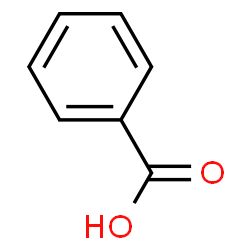
\includegraphics[width=0.1\textwidth]{img/acbenz.png}}
{\label{fig:2}}
\end{figure}

\textit{Aliquam erat nulla, suscipit id dignissim molestie, eleifend quis tortor. Pellentesque tempus egestas orci, sit amet eleifend elit condimentum id. Etiam id nisi velit. Etiam mauris nisl, facilisis sed egestas nec, tempor a est. In eget lacus vitae velit volutpat maximus. Vestibulum maximus arcu sit amet lacus maximus consequat. Duis sodales libero non metus finibus, eget ornare sem consequat.}

\begin{wrapfigure}{r}{0.3\textwidth} %this figure will be at the right
    \centering
    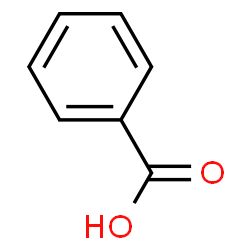
\includegraphics[scale=0.5]{img/acbenz.png}
    \caption{Didascalia dell'immagine sulla destra circondata da testo.} 
    \label{fig:3}
\end{wrapfigure}

\textit{Nullam vel lorem porttitor, convallis ex eget, condimentum velit. Integer sed sem aliquet, elementum ipsum in, rutrum elit. Vestibulum in arcu eget odio egestas varius. Vivamus lacus augue, dignissim at arcu a, consequat iaculis leo. Nam sit amet varius tellus. Nulla tempor velit nibh, et tincidunt diam porta vel. Mauris sit amet erat ut neque vehicula ultrices et eu sem. Phasellus pellentesque ultricies sapien. Curabitur at sodales mauris, maximus auctor mi. Vestibulum semper mauris in euismod rutrum. Fusce pellentesque in mi ac euismod.}

\textit{Nam gravida magna ut volutpat placerat. Pellentesque habitant morbi tristique senectus et netus et malesuada fames ac turpis egestas. Sed consequat justo condimentum metus bibendum mattis. Etiam id euismod ante. Nam sit amet ex libero. Proin id mauris at neque pellentesque accumsan eu ut ligula. Vivamus sodales magna sed risus faucibus tincidunt in eu felis.}

\begin{figure}
    \centering
    
\includegraphics[scale=0.2]{img/pittogrammi/Acute toxicity.png}
    
\includegraphics[scale=0.2]{img/pittogrammi/Explosive.png}
    \caption{Figure affiancate al centro della pagina nella posizione decisa da LaTex}
    \label{fig:4}
\end{figure}

\textit{Vivamus sit amet suscipit turpis, at eleifend risus. Vestibulum ante ipsum primis in faucibus orci luctus et ultrices posuere cubilia curae; Curabitur eget pharetra est, in mattis erat. Aenean pharetra finibus posuere. Nullam ipsum lacus, molestie nec eros eu, lacinia facilisis augue. Aenean dapibus rhoncus mi ut vulputate. Mauris commodo ultricies nulla egestas porttitor.}

\begin{figure}[h]
    \centering
    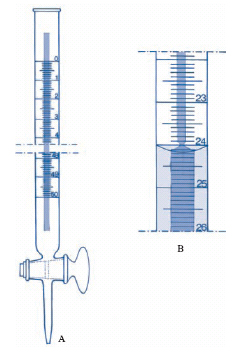
\includegraphics{img/buretta.jpg}
    \caption{Buretta}
    \label{fig:5}
\end{figure}

\begin{figure}[h!]
     \centering
     \begin{subfigure}[b]{0.29\textwidth}
         \centering
         \includegraphics[width=\textwidth]{img/cipolla_safranina.jpg}
         \caption{Cipolla con safranina}
         \label{fig:y equals x}
     \end{subfigure}
     \hfill
     \begin{subfigure}[b]{0.29\textwidth}
         \centering
         \includegraphics[width=\textwidth]{img/patata_H2O.jpg}
         \caption{Buccia di patata con acqua}
         \label{fig:three sin x}
     \end{subfigure}
     \hfill
     \begin{subfigure}[b]{0.29\textwidth}
         \centering
         \includegraphics[width=\textwidth]{img/carota_H2O.jpg}
         \caption{Carota in acqua}
         \label{fig:five over x}
     \end{subfigure}
        \label{fig:three graphs}
\end{figure}

\newpage
\subsection*{Formule chimiche}
\begin{figure}[!ht]
    \chemfig{O=H}
\end{figure}

\begin{figure}[!ht]
    \chemfig{A-[1]B-[7]C}
    \caption{To define chemical formulae you can use units that define the angles}
\end{figure}

\begin{figure}[!ht]
    \chemfig{A-[:50]B-[:-25]C}
    \caption{Absolute angles}
\end{figure}


\begin{figure}[!ht]
    \chemfig{A-[::50]B-[::-25]C}
    \caption{Relative angles}
\end{figure}


\begin{figure}[!ht]
    \chemfig{A*5(-B=C-D-E=)}
    \caption{Regular polygons}
\end{figure}

\begin{figure}[!ht]
    \chemfig{A*5(-B=C-D)}
    \caption{Incomplete rings are also possible}
\end{figure}

\begin{figure}[!ht]
    \chemfig{H-C(-[2]H)(-[6]H)-C(=[1]O)-[7]H}
    \caption{Branched molecule}
\end{figure}

\begin{figure}
    \chemfig{A*6(-B=C(-CH_3)-D-E-F(=G)=)}
    \caption{Branched ring}
\end{figure}

\begin{figure}[!ht]
{\huge 
    \setchemfig{atom sep=2em,bond style={line width=1pt,red,dash pattern=on 2pt off 2pt}}  
    \chemname
    {\chemfig{H-C(-[2]H)(-[6]H)-C(=[1]O)-[7]H}}    
    {Ethanal}
}
\end{figure}

\newpage
\subsection*{Molecular orbital diagrams}
\begin{figure}[!ht]
        \begin{modiagram}
        \atom{left}{1s, 2s, 2p}
        \end{modiagram}
    \caption{First molecular orbital diagrams}
\end{figure}

\begin{figure}[!ht]
\begin{modiagram}
 \atom{right}{
    1s = { 0; pair} ,
    2s = { 1; pair} ,
    2p = {1.5; up, down }
 }


 \atom{left}{
    1s = { 0; pair} ,
    2s = { 1; pair} ,
    2p = {1.5; up, down }
 }
 \end{modiagram}
 \end{figure}

\begin{figure}[!ht]
 \begin{modiagram}
 \atom{left}{1s}
 \atom{right}{1s={;up}}
 \molecule{
    1sMO={0.75;pair,up}
  }
\end{modiagram}
\end{figure}

\begin{figure}[!ht]
\begin{modiagram}
 \atom{left}{
      1s, 2s, 2p = {;pair,up,up}
  }
  \atom{right}{
      1s, 2s, 2p = {;pair,up,up}
  }
  \molecule{
      1sMO, 2sMO, 2pMO = {;pair,pair,pair,up,up}
  }
\end{modiagram}
\end{figure}

\begin{figure}[!ht]
\begin{modiagram}
 \atom{left}{1s}
 \atom{right}{1s={;up}}
 \molecule{
    1sMO={;pair,up}
 }
 \draw[<-,shorten <=8pt,shorten >=15pt,blue]
 (1sigma*) --++(2,1) node {anti-bonding MO};
\end{modiagram}
\end{figure}

\newpage
\subsection*{Flowchart}
Ecco invece un esempio di flowchart che potrebbe essere utile in certi procedimenti particolarmente articolati.
\begin{figure}[!ht]
    \begin{center}
        \begin{tikzpicture}[node distance=2cm] % per guida -> https://it.overleaf.com/learn/latex/LaTeX_Graphics_using_TikZ%3A_A_Tutorial_for_Beginners_(Part_3)%E2%80%94Creating_Flowcharts
            \node (start) [starter] {Inizio};
            \node (in1) [io, below of=start] {Ingresso};
            \node (pro1) [process, below of=in1] {Processo 1};
            \node (dec1) [decision, below of=pro1,  yshift=-0.5cm] {Decisione 1};
            \node (pro2a) [process, below of=dec1, yshift=-0.5cm] {Process 2a};
            \node (pro2b) [process, right of=dec1, xshift=2cm] {Process 2b};
            \node (out1) [io, below of=pro2a] {Output};
            \node (proc3a) [process, right of=out1, xshift=2cm] {Process 3a};
            \node (process_longtext2) [process_longtext2.5, right of=proc3a , xshift=2cm, yshift=2cm]{Lorem ipsum dolor sit amet, consectetur adipiscing elit. Suspendisse euismod interdum ornare.};
            \node (stop) [terminator, below of=out1] {Stop};
            
            \draw [arrow_stealth] (start) -- (in1);
            \draw [arrow_stealth] (in1) -- (pro1);
            \draw [arrow_stealth] (pro1) -- (dec1);
            \draw [arrow_stealth] (dec1) -- node[anchor=east] {yes} (pro2a);
            \draw [arrow_stealth] (dec1) -- node[anchor=south] {no} (pro2b);
            \draw [arrow_stealth_rounded] (pro2b) |- (pro1); %per fare linea segmentata
            \draw [arrow_latex] (pro2a) -- (out1);
            \draw [line_rect] (out1) -- (proc3a);
            \draw [duble_arrow_latex] (proc3a) -- (process_longtext2);
            \draw [duble_arrow_latex] (process_longtext2) |- (stop);
            \draw [arrow_latex] (out1) -- (stop);
        \end{tikzpicture}
    \end{center}
\end{figure}

\newpage
\subsection*{Note e appunti vari}
Lorem ipsum dolor sit amet, consectetur adipiscing elit. Sed eget velit ullamcorper, convallis neque eget, tempus leo. Aenean eget est ornare, mattis turpis sit amet, vestibulum ante.\unsure{Change this!} Integer quis molestie arcu. Duis sem felis, posuere ut ante vitae, lobortis tincidunt dolor. Ut aliquet nunc sed lorem vehicula, ac tristique velit venenatis. Aliquam feugiat interdum magna, luctus sodales velit porta et. Nunc varius lorem nec varius malesuada. Praesent ante nisi, ultrices et venenatis sed, commodo vitae eros.\change{Change this!}

Pellentesque consectetur malesuada lectus, ut faucibus diam egestas ac. Aenean porttitor at libero a venenatis. Morbi sollicitudin, leo sed pellentesque facilisis, lacus diam lobortis tellus, sit \info{This can help me in chapter seven!}amet vulputate turpis sem id ipsum. Nunc ac aliquet mi, non porta quam. Maecenas auctor pulvinar sodales. Suspendisse eget mi arcu. Mauris quis nulla sit amet risus dapibus eleifend sed eget purus. Pellentesque libero nunc, \improvement{This really needs to be improved!\newline\newline What was I thinking?!}congue vitae mi sit amet, lobortis faucibus ante. Vestibulum cursus, neque quis auctor laoreet, sapien risus vestibulum orci, a rutrum tellus nisl quis ligula.

Sed non erat metus. Donec aliquet ex non neque sodales pretium. Aliquam eu sapien elit. Aliquam finibus felis et neque elementum, laoreet tempus urna auctor. Vivamus ac congue elit, vitae volutpat nulla. Sed pretium in lorem eget porttitor. Etiam interdum euismod odio, quis sollicitudin tellus rutrum et. Proin consequat, risus at consequat elementum, turpis elit tincidunt tellus, eu finibus dui mi vel eros. Donec in nulla tortor. Maecenas mollis consectetur erat sed elementum. Pellentesque habitant morbi tristique senectus et netus et malesuada fames ac turpis egestas. Nunc ultrices enim ut risus scelerisque, sed ultrices nibh congue. Mauris volutpat, elit vel sagittis consequat, lorem sapien iaculis sapien, id faucibus purus eros ut mauris. Vestibulum ornare elementum pretium.

Nunc non ante suscipit, dictum justo nec, dapibus elit. Proin lacinia leo fermentum dui bibendum, ac pellentesque felis malesuada. Integer sollicitudin tempor varius. Quisque sed magna rhoncus, ultricies nisi a, sollicitudin quam. Curabitur ut tempor lectus. Donec iaculis condimentum vehicula. In convallis ac sapien vel aliquam. Orci varius natoque penatibus et magnis dis parturient montes, nascetur ridiculus mus. Suspendisse ac eleifend dolor, at scelerisque urna. Quisque ac facilisis erat. Etiam accumsan risus sed molestie pulvinar. Orci varius natoque penatibus et magnis dis parturient montes, nascetur ridiculus mus. Proin non turpis non felis pretium convallis.
\improvement[inline]{The following section needs to be rewritten!}

Sed finibus pellentesque diam, et sagittis tortor ultrices ut. Orci varius natoque penatibus et magnis dis parturient montes, nascetur ridiculus mus. Suspendisse volutpat ullamcorper dui in cursus. Proin ullamcorper neque posuere porttitor rutrum. Suspendisse ac tortor justo. Vivamus convallis ligula at lacus commodo, eu mattis nulla vehicula. Vestibulum interdum leo et volutpat rhoncus.
\thiswillnotshow{This is hidden since option `disable' is chosen!}

E ora aggiungo una lista delle note.
\listoftodos[Notes to address] %parte di esempi per immagini o formule, elimina pure dopo aver scritto la relazione.
\end{document}
